\chapter{Fysieke beveiliging met een Web Of Trust}
\label{ch:fysieke-beveiliging-met-een-wot}

Fysieke beveiliging is het gebruik van fysieke componenten om een plaats,
gebouw, kamer of andere fysieke activa, te beschermen. Fysieke beveiliging kan
gebruik maken van camera’s, bewegingsdetectoren, hangsloten, poorten, deuren en
ook beveiligingspersoneel \autocite{FennellyPhysicalSecurity}. Een Web Of Trust
is gemaakt om de identiteit van een individu te bevestigen en het individu op
manier dan te authenticeren. Voor een toepassing van het Web Of Trust in de
fysieke beveiliging wordt dus gefocust op toestellen of middelen die deze rol
vervullen. Enkele voorbeelden hiervan zijn deuren en poorten.

Toegang restricterende middelen zoals deuren en poorten gebruiken vaak
magneetkaarten, digitale pasjes en soms zelf biometrische eigenschappen zoals
vingerafdrukken van individuen om deze te identificeren. De biometrische
authenticatie heeft als voordeel dat een impersonatie van een individu bijzonder
moeilijk wordt sinds biometrische eigenschappen uniek zijn per individu. De
magneetkaarten en digitale pasjes kunnen daarom ook gecomplementeerd worden met
pincodes of wachtwoorden om de mogelijkheid dat iemand binnen kan met een ander
persoon zijn of haar kaart, te verminderen. De toerekenbaarheid die we moeten
kunnen bewijzen vereist dat als een individu zich authentiseert aan een deur, we
uit de logs moeten kunnen bewijzen dat dit inderdaad door een bepaalde persoon
gedaan was.

Natuurlijk moet elke medewerker niet in alle plaatsen binnen kunnen. Hierdoor is
het vereist dat elke medewerker specifieke toegangsregels kan gegeven worden.

\section{Fysieke toegangscontrole met complementerende beveiliging}
\label{sec:fysieke-toegangscontrole-met-complementerende-beveiliging}

Stel, de private sleutel van de medewerker wordt geplaatst op een elektronische
kaart. De medewerker moet zijn wachtwoord ingeven om het authenticatieproces te
doorlopen. Er zijn direct twee grote problemen met deze aanpak. Het eerste
probleem is dat de private sleutel nu op een ID kaart staat zonder enige vorm
van beveiliging. Wanneer de kaart verloren gaat, is het wachtwoord van de
private sleutel het enige dat het sleutelpaar nog beschermt tegen ongeoorloofde
toegang. Het tweede probleem, is dat het ingeven van een wachtwoord van minstens
zestien tekens en dat complexe karakters kan bevatten zeer tijdrovend zal zijn.

Een betere manier zou zijn om een apart sleutelpaar te gebruiken voor fysieke
toegang. Het wachtwoord dat de private sleutel van dit nieuwe sleutelpaar
beveiligd kan beperkt worden tot getallen. Om duidelijk te maken dat het
sleutelpaar behoort tot een bepaalde medewerker kan deze medewerker de nieuwe
publieke sleutel ondertekenen met zijn of haar huidige sleutel. Deze nieuwe
private sleutel kan dan geplaatst worden op de elektronische kaart waarna bij
authenticatie een toegangsbericht wordt ondertekend bij ingave van het
wachtwoord van de private sleutel. Deze structuur kan teruggevonden worden in
figuur \ref{fig:physical-security-key-structure}. Het authenticatieproces kan
teruggevonden worden in figuur \ref{fig:physical-security-auth-proces}

\begin{figure}[H]
	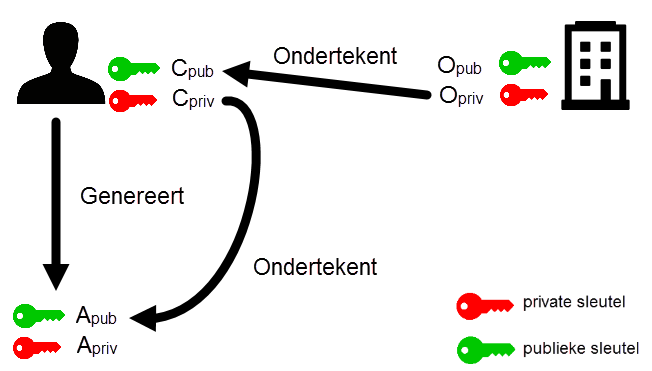
\includegraphics[width=\textwidth,keepaspectratio]{img/physical-security-key-diagram.png}
	\centering
	\caption{Een sleutel structuur met extra persoonlijke sleutel}
	\label{fig:physical-security-key-structure}
\end{figure}

\begin{figure}[H]
	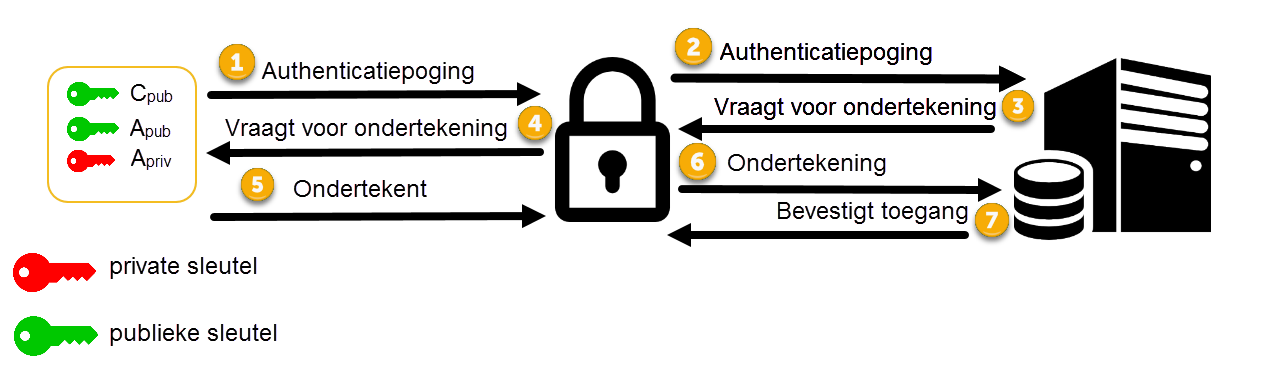
\includegraphics[width=\textwidth,keepaspectratio]{img/physical-security-auth-process.png}
	\centering
	\caption{Een sleutel structuur met extra persoonlijke sleutel}
	\label{fig:physical-security-auth-proces}
\end{figure}

In stap één scant de gebruiker de elektronische kaart. De sleutels op de kaart,
C\textsubscript{pub}, A\textsubscript{pub} en A\textsubscript{priv} worden
doorgestuurd naar de server. De server controleert of C\textsubscript{pub} door
de hoofdsleutel(s) ondertekend is, en de sleutel niet teruggetrokken is.
Vervolgens controleert de server of A\textsubscript{pub} ondertekent is door het
sleutelpaar C.
Indien dit zo is, zal de server een bericht genereren dat een timestamp bevat.
Hierna, in stap drie en vier, zal de server vragen om dit bericht te
ondertekenen. Het individu dat zich nu wilt authenticeren moet zijn of haar PIN
ingeven. De PIN ontgrendelt de private sleutel en ondertekent het gegeven
bericht dat na succesvolle ondertekening na de server wordt teruggestuurd (stap
vijf en zes). In stap zeven controleert de server of de ondertekening correct
is. Indien dit het geval is, betekent dit dat de gebruiker geauthenticeerd is.
Er moet nog een controle gedaan worden op autorisatie. De server controleert nu
of de gebruiker toegang heeft tot de gevraagde plaats. Wanneer dit het geval is
zal de server het toegangsapparaat signaleren om de deur open te doen.

Het is belangrijk om dit te doen nadat het individu geauthenticeerd is. Dit
voorkomt namelijk dat een aanvaller controleert of een bepaalde kaart toegang
heeft tot een plaats zonder een PIN in te geven.

Er is nog één probleem dat moet opgelost worden. De private sleutel wordt
momenteel nog altijd op de badge opgeslagen zonder enige vorm van beveiliging.
Dit betekent dat enkel een PIN de private sleutel beschermt. Een mogelijke
oplossing is een speciaal sleutelpaar aanmaken waarvan de private sleutel op de
access control server staat. De A\textsubscript{priv} sleutel wordt vervolgens
versleuteld met de publieke sleutel van de access control server en
geëncrypteerd opgeslagen op de badge. Bij authenticatie wordt
A\textsubscript{priv} tijdelijk gedecrypteerd voor de handtekening te kunnen
verrichten.

\subsection{Verlies van een badge}

Indien een badge verloren gaat, moet de publieke sleutel die de gebruiker in de
acces control server paart, opgezocht worden en gemarkeerd worden als inactief.
Ook moet het sleutelpaar dat zich op de badge bevond, teruggetrokken worden. De
verloren badge is nu waardeloos voor een potentiële aanvaller. De stappen voor
een nieuwe badge aan te maken worden vervolgens doorlopen.

Indien de badge nog teruggevonden wordt, kan deze leeggemaakt worden en opnieuw
gebruikt.

\section{Fysieke toegangscontrole zonder complementeerde beveiliging}

Het is vaak niet nodig om extra beveiliging zoals PIN of biometrische
authenticatie toe te voegen. Zo’n systeem heeft als voordeel dat er geen tijd
moet worden geïnvesteerd in de extra beveiligingen. Een voorbeeld van een
omgeving waarin dit systeem geprefereerd wordt is bijvoorbeeld een ziekenhuis.
Dit komt door het feit dat in een omgeving zoals een ziekenhuis, snelheid
kritiek is \autocite{Podevyn}. Het aanmaken van dit soort badge staat beschreven
in figuur \ref{fig:electronic-card-creation-no-pin}.

\begin{figure}[H]
	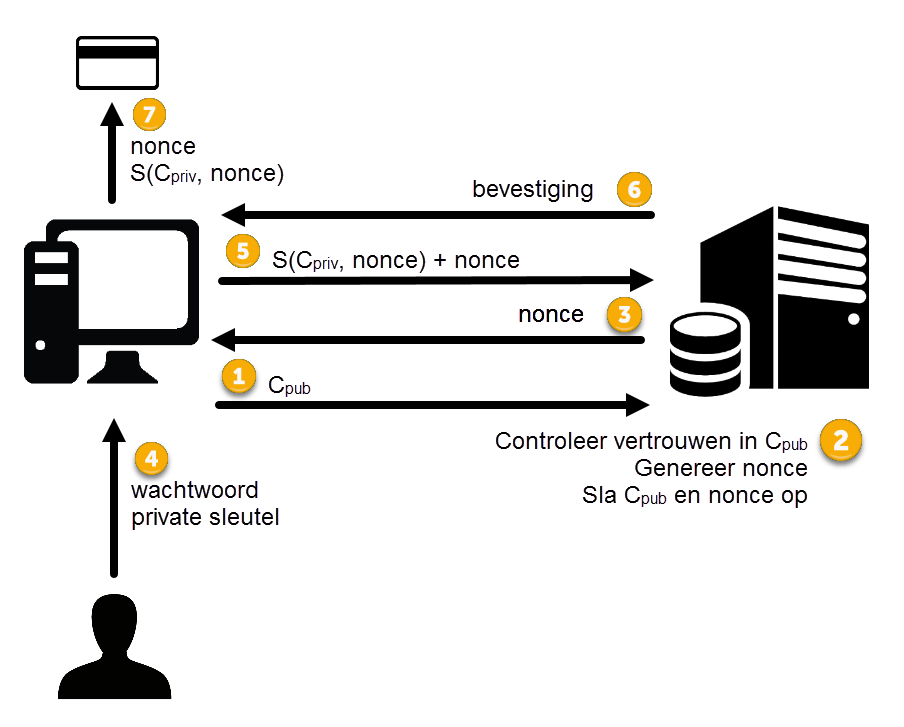
\includegraphics[width=\textwidth,keepaspectratio]{img/electronic-card-creation-no-pin.png}
	\centering
	\caption{Het aanmaken van een ID kaart zonder complementerende beveiliging}
	\label{fig:electronic-card-creation-no-pin}
\end{figure}

Het proces heeft een beginstructuur waarbij de medewerker een badge aangesloten
heeft op de computer waarop hij of zij werkt. De private en publieke sleutel van
de medewerker zijn bereikbaar.

De computer stuurt de publieke sleutel naar de access control server. Deze gaat
na of de publieke sleutel vertrouwd wordt door de hoofdsleutel(s). Hierna
creëert de server een nonce, een unieke willekeurige waarde. De server bewaart
deze nonce samen met de publieke sleutel. Hierna zendt de server de nonce naar
de medewerker zijn of haar computer. De medewerker ondertekent nu de nonce met
zijn of haar private sleutel. Deze bewerking is terug te vinden onder
S(C\textsubscript{priv}, nonce) waarbij S een \textit{sign} methode is, de
eerste parameter gelijk is aan de gebruikte sleutel en de tweede parameter
gelijk aan het bericht. Deze handtekening en nonce worden verstuurd naar de
server. Deze zoekt naar de opgeslagen nonce en valideert de handtekening
vervolgens met de opgeslagen publieke sleutel. Indien deze correct zijn, wordt
dit bevestigd aan het werkstation van de medewerker. Hierna wordt de nonce en de
handtekening ervan op de badge opgeslagen.

Wanneer de medewerker zich authenticeerd bij een fysiek toegang controlerend
systeem, scant hij de badge. De nonce en S(C\textsubscript{priv}, nonce) worden
doorgestuurd naar de server. De server doet een lookup van de nonce. Vervolgens
controleert de server of de publieke sleutel die gevonden is tijdens de lookup,
de S(C\textsubscript{priv}, nonce) kan valideren. Indien dit het geval is, dan
is de medewerker geauthenticeerd. De autorisatie gebeurt op dezelfde manier als
in hoofdstuk
\ref{sec:fysieke-toegangscontrole-met-complementerende-beveiliging}.

\subsection{Verlies van een badge}

Indien een badge verloren gaat, moet de publieke sleutel die de gebruiker in de
acces control server paart, opgezocht worden en gemarkeerd worden als inactief.
De stappen voor een nieuwe badge aan te maken worden vervolgens doorlopen.

Indien de badge nog teruggevonden wordt, kan deze leeggemaakt worden en opnieuw
gebruikt.

\subsection{Voor- en nadelen}
Het voordeel van deze aanpak is dat de private sleutel nooit de veiligheid van
het werkstation van de medewerker verlaat. Het nadeel echter is dat iedereen die
de badge kan bemachtigen, deze kan misbruiken tot het verlies van de kaart
bekend is geworden en er correct naar gehandeld is. Dit wordt gedeeltelijk
gecompenseerd door het feit dat het terugtrekken van de badges minder stappen
vereist.

\section{Access control server}
De access control server heeft als taak om de toegang van alle medewerkers
centraal te beheren. De server heeft enkele gegevens nodig om te kunnen werken.
Hieronder vallen onder andere alle apparaten, deuren, enzovoort die onder access
control vallen. Verder wordt natuurlijk bijgehouden welke personen toegang
hebben welke plaatsen. Een persoon wordt geïdentificeerd aan de hand van een
publieke sleutel.
